\documentclass[aspectratio=169,11pt]{beamer}

\usepackage[T1]{fontenc}
\usepackage{lmodern}
\usepackage{amsmath,amssymb,mathtools,bm}
\usepackage{booktabs,array}
\usepackage{graphicx}
\usepackage{ragged2e}
\usepackage{pgfpages}
\usepackage{appendixnumberbeamer}

% Keep Beamer's translated appendix label out of the PDF bookmark command.
\pdfstringdefDisableCommands{\def\translate#1{#1}}

% Set this switch to \showspeakernotestrue to compile slides with notes on the right.
\newif\ifshowspeakernotes
\showspeakernotesfalse
\ifshowspeakernotes
  \setbeameroption{show notes on second screen=right}
\else
  \setbeameroption{hide notes}
\fi

\graphicspath{{presentation_assets/}}

\definecolor{ink}{HTML}{102A43}
\definecolor{blue}{HTML}{1769AA}
\definecolor{orange}{HTML}{D86B27}
\definecolor{teal}{HTML}{247B7B}
\definecolor{mist}{HTML}{EEF4F8}
\definecolor{muted}{HTML}{52606D}

\setbeamercolor{normal text}{fg=ink,bg=white}
\setbeamercolor{structure}{fg=blue}
\setbeamercolor{frametitle}{fg=ink,bg=white}
\setbeamercolor{title}{fg=white}
\setbeamercolor{subtitle}{fg=white!82!blue}
\setbeamercolor{author}{fg=white!88!blue}
\setbeamercolor{date}{fg=white!72!blue}
\setbeamercolor{alerted text}{fg=orange}

\setbeamertemplate{navigation symbols}{}
\setbeamertemplate{itemize item}{\color{orange}\small$\blacktriangleright$}
\setbeamertemplate{itemize subitem}{\color{blue}\scriptsize$\bullet$}
\setbeamertemplate{frametitle}{%
  \vspace{0.18cm}\insertframetitle\par
  \vspace{-0.10cm}{\color{blue}\rule{\textwidth}{0.7pt}}
}
\setbeamertemplate{footline}{%
  \leavevmode%
  \hbox{%
    \begin{beamercolorbox}[wd=.82\paperwidth,ht=2.8ex,dp=1.2ex,leftskip=.55cm]{author in head/foot}%
      \color{muted}\scriptsize Financial SDEs: GBM benchmark and non-affine volatility
    \end{beamercolorbox}%
    \begin{beamercolorbox}[wd=.18\paperwidth,ht=2.8ex,dp=1.2ex,rightskip=.55cm plus1fil]{date in head/foot}%
      \color{muted}\scriptsize \insertframenumber/\inserttotalframenumber
    \end{beamercolorbox}%
  }
}

\setbeamerfont{title}{size=\fontsize{25}{29}\selectfont,series=\bfseries}
\setbeamerfont{subtitle}{size=\large}
\setbeamerfont{frametitle}{size=\fontsize{20}{23}\selectfont,series=\bfseries}
\setbeamerfont{normal text}{size=\fontsize{11}{14}\selectfont}

\newcommand{\E}{\mathbb E}
\newcommand{\Var}{\operatorname{Var}}
\newcommand{\dd}{\,\mathrm d}
\newcommand{\source}[1]{\par\vspace{0.06cm}{\color{muted}\tiny Source: #1}}

\title{Financial SDEs}
\subtitle{GBM benchmark and non-affine volatility}
\author{Numerical Analysis of ODEs and PDEs}
\date{Project 1 Presentation}

\begin{document}

{
\setbeamertemplate{footline}{}
\setbeamercolor{background canvas}{bg=ink}
\begin{frame}[plain]
  \vspace{0.30cm}
  {\color{white!82!blue}\large\bfseries MTH321\par}
  \vspace{0.12cm}
  {\color{white!65!blue}\small Numerical Analysis of ODEs and PDEs\par}
  \vspace{0.20cm}
  {\color{orange}\rule{1.3cm}{1.4pt}\par}
  \vfill
  {\usebeamerfont{title}\color{white}\inserttitle\par}
  \vspace{0.25cm}
  {\usebeamerfont{subtitle}\color{white!82!blue}\insertsubtitle\par}
  \vfill
  {\color{white!70!blue}\small \insertdate}
  \vspace{0.25cm}
\end{frame}
}
\note{
Good morning. Our project studies two financial stochastic differential equations. GBM gives us an exact pathwise benchmark, so it tells us whether the numerical methods are implemented correctly. The non-affine stochastic-volatility model removes that exact solution and forces us to build and test a numerical reference. That change is the main story of the presentation.
}

\begin{frame}{Anatomy of a stochastic differential equation}
\begin{columns}[T,onlytextwidth]
\column{0.57\textwidth}
\vspace{0.15cm}
\[
  \dd X_t = \underbrace{a(t,X_t)\dd t}_{\text{drift}}
  + \underbrace{b(t,X_t)\dd W_t}_{\text{diffusion}}
\]
\vspace{0.15cm}
\[
  \Delta W_n = \sqrt{\Delta t}\,Z_n,
  \qquad Z_n\sim N(0,1)
\]
\[
  \text{GBM:}\qquad \dd S_t=\mu S_t\dd t+\sigma S_t\dd W_t.
\]

\column{0.43\textwidth}
\textbf{Local interpretation}
\begin{align*}
\E[\dd X_t\mid\mathcal F_t] &= a(t,X_t)\dd t,\\
\Var(\dd X_t\mid\mathcal F_t) &= b(t,X_t)^2\dd t.
\end{align*}
\begin{itemize}
  \item Drift controls the conditional mean movement.
  \item Diffusion controls the size of short-time random movement.
\end{itemize}
\end{columns}
\end{frame}
\note{
An SDE has two parts. The drift is the conditional mean rate of change. The diffusion determines the conditional variance over a short interval. Brownian increments are proportional to the square root of the time step, not the time step itself. This scaling is why stochastic methods have strong orders such as one half. It also explains why we need It\^o calculus instead of ordinary calculus.
}

\begin{frame}{It\^o's formula and the exact GBM solution}
\footnotesize
\setlength{\abovedisplayskip}{4pt}
\setlength{\belowdisplayskip}{4pt}
\textbf{It\^o's formula:} if $\dd S_t=a(t,S_t)\dd t+b(t,S_t)\dd W_t$
and $f\in C^{1,2}$, then
\[
 \boxed{\dd f(t,S_t)=\left(f_t+a f_S+\tfrac12b^2f_{SS}\right)\dd t
 +b f_S\dd W_t.}
\]
\begin{columns}[T,onlytextwidth]
\column{0.48\textwidth}
\textbf{Apply it to GBM}
\[
 \dd S_t=\mu S_t\dd t+\sigma S_t\dd W_t.
\]
For $f(S)=\log S$, $f_t=0$, $f_S=1/S$, $f_{SS}=-1/S^2$:
\begin{align*}
 \dd\log S_t
 &=\left(\mu S_t\frac1{S_t}
 -\frac12\sigma^2S_t^2\frac1{S_t^2}\right)\dd t
 +\sigma\dd W_t\\
 &=\left(\mu-\tfrac12\sigma^2\right)\dd t+\sigma\dd W_t.
\end{align*}
\column{0.48\textwidth}
\textbf{Integrate and exponentiate}
\[
 \log S_t=\log S_0+(\mu-\tfrac12\sigma^2)t+\sigma W_t.
\]
\[
 \boxed{S_t=S_0e^{(\mu-\sigma^2/2)t+\sigma W_t}.}
\]
\begin{align*}
 \E[S_T]&=S_0e^{\mu T},\\
 \Var(S_T)&=S_0^2e^{2\mu T}(e^{\sigma^2T}-1).
\end{align*}
The terminal law is lognormal; $S_t>0$ for $S_0>0$.
\end{columns}
\end{frame}
\note{
The boxed equation at the top is It\^o's formula. Compared with an ordinary chain rule, it includes a second-derivative term from Brownian quadratic variation. For GBM, substitute a equal to mu S and b equal to sigma S. Choose f equal to log S, whose first derivative is one over S and second derivative is minus one over S squared. Substitution gives drift mu minus one half sigma squared and diffusion sigma. Integrating and exponentiating produces the exact GBM solution on the right. Its terminal law is lognormal and its price remains positive. Mu is the expected growth parameter under the chosen measure.
}

\begin{frame}{It\^o--Taylor expansion: which terms are retained?}
\small
For $\dd U_t=a(U_t)\dd t+b(U_t)\dd W_t$, write
$a_n=a(U_n)$, $b_n=b(U_n)$, and $b'_n=b'(U_n)$.
\medskip

\textbf{Scalar It\^o--Taylor expansion (terms used by the two methods):}
\[
 U_{t_{n+1}}=U_n+a_nh+b_n\Delta W_n
 +\tfrac12b_nb'_n\bigl[(\Delta W_n)^2-h\bigr]+R_n.
\]
\textbf{Euler--Maruyama: retain $a_nh$ and $b_n\Delta W_n$.}
\[
 \boxed{U_{n+1}^{\mathrm{EM}}=U_n+a_nh+b_n\Delta W_n.}
\]
\textbf{Milstein: also retain the next stochastic correction.}
\[
 \boxed{U_{n+1}^{\mathrm{Mil}}=U_n+a_nh+b_n\Delta W_n
 +\tfrac12b_nb'_n\bigl[(\Delta W_n)^2-h\bigr].}
\]
$R_n$ collects the omitted terms. The correction follows from
$\int_{t_n}^{t_{n+1}}(W_s-W_{t_n})\dd W_s
 =\tfrac12[(\Delta W_n)^2-h]$.
\end{frame}
\note{
The top equation shows the scalar It\^o--Taylor terms relevant to these methods. EM keeps the drift term and the first Brownian term. Milstein keeps the same terms plus the correction containing b times its derivative. The remainder collects the terms omitted from this displayed expansion. The distinction between the methods is therefore the correction, and whether it vanishes depends on the diffusion derivative.
}

\begin{frame}{Log-price GBM: why EM and Milstein coincide}
\small
For $X_t=\log S_t$, It\^o's formula gives
\[
 \dd X_t=(\mu-\tfrac12\sigma^2)\dd t+\sigma\dd W_t.
\]
\textbf{Substitute the coefficients into the two methods:}
\[
 a(X)=\mu-\tfrac12\sigma^2,\qquad
 b(X)=\sigma\ \text{(constant)},\qquad \boxed{b'(X)=0.}
\]
\begin{align*}
 X_{n+1}^{\mathrm{EM}}&=X_n+(\mu-\tfrac12\sigma^2)h+\sigma\Delta W_n,\\
 X_{n+1}^{\mathrm{Mil}}&=X_n+(\mu-\tfrac12\sigma^2)h+\sigma\Delta W_n
 +\underbrace{\tfrac12\sigma\cdot0\bigl[(\Delta W_n)^2-h\bigr]}_{=0}.
\end{align*}
\textbf{Both give the same exact grid update.}
\medskip

For the original price equation, $b(S)=\sigma S$ and $b'(S)=\sigma$:
$bb'=\sigma^2S\ne0$ when $\sigma\ne0$ and $S>0$.
We therefore compare EM and Milstein in price space.
\end{frame}
\note{
For log-price GBM, the drift and diffusion are constant. In particular, b equals sigma, so its derivative is zero. Substitution into Milstein makes the additional correction zero. EM and Milstein therefore have the same update, which is also the exact grid transition in this constant-coefficient case. For the original price equation, b equals sigma times S, so its derivative is sigma rather than zero. The correction remains. This is why we use price-space GBM to compare the methods.
}

\begin{frame}{Strong and weak convergence answer different questions}
\begin{columns}[T,onlytextwidth]
\column{0.48\textwidth}
\textbf{Strong error}
\[
\E\left|S_T^{(h)}-S_T\right|\le Ch^p
\]
Same Brownian path for the numerical and exact solutions.
\[
p_{\mathrm{EM}}=\tfrac12,
\qquad p_{\mathrm{Mil}}=1.
\]

\column{0.48\textwidth}
\textbf{Weak error}
\[
\left|\E\phi(S_T^{(h)})-\E\phi(S_T)\right|\le Ch^q
\]
For smooth observables, both methods have $q=1$.
For the GBM mean,
\[
\E[S_N]=S_0(1+\mu h)^{T/h}
=S_0e^{\mu T}+O(h).
\]
\end{columns}
\end{frame}
\note{
Strong and weak convergence are not interchangeable. Strong error compares two solutions driven by the same Brownian path. It matters when the path itself matters. Weak error compares expectations of observables. Both EM and Milstein have weak order one under the standard smoothness assumptions. For the mean of GBM, we can prove this directly because both discrete schemes have the same expected one-step multiplier, one plus mu h. Expanding that exact discrete expectation gives a first-order bias. Since the bias becomes small, we use paired differences, confidence intervals, and many paths so Monte Carlo noise does not hide it.
}

\begin{frame}{Strong convergence: calculation}
\scriptsize
\setlength{\abovedisplayskip}{4pt}
\setlength{\belowdisplayskip}{4pt}
\textbf{1. Fix $T$, choose $h=T/N$, and generate $M$ independent paths:}
\[
 \Delta W_n^{(m)}=\sqrt h\,Z_n^{(m)},\qquad Z_n^{(m)}\sim N(0,1).
\]
\textbf{2. Compute numerical and exact prices on the same Brownian path:}
\begin{align*}
 S_{n+1}^{\mathrm{EM}}&=S_n^{\mathrm{EM}}(1+\mu h+\sigma\Delta W_n),\\
 S_{n+1}^{\mathrm{Mil}}&=S_n^{\mathrm{Mil}}\left[1+\mu h+\sigma\Delta W_n
 +\tfrac12\sigma^2((\Delta W_n)^2-h)\right],\\
 S_T&=S_0\exp\!\left[(\mu-\tfrac12\sigma^2)T+\sigma\sum_n\Delta W_n\right].
\end{align*}
\textbf{3. Estimate terminal $L^1$ strong error (absolute value before averaging):}
\[
 e_s(h)=\E|S_{T,h}-S_T|,\qquad
 \widehat e_s(h)=\frac1M\sum_{m=1}^M|S_{T,h}^{(m)}-S_T^{(m)}|.
\]
\textbf{4. Halve $h$ repeatedly; couple grids by summing fine increments:}
\[
 e_s(h)\approx C_sh^{p_s}\ \Longrightarrow\
 \widehat p_s=\frac{\log[\widehat e_s(h)/\widehat e_s(h/2)]}{\log2}.
\]
\end{frame}
\note{
Strong convergence asks whether the approximate price approaches the exact price on the same Brownian path. First fix the final time and choose a grid. Generate independent Brownian increments for each simulated path. Starting from S zero, iterate EM or Milstein. Use the sum of those very same increments in the exact GBM formula. Take the absolute terminal difference for each path, then average. Repeat with halved time steps, coupling grids by summing fine increments. If the error is proportional to h to the power p, the logarithm of the error ratio divided by log two estimates p. In practice we fit several grids. This is an empirical order estimate, while a convergence theorem establishes a bound under stated assumptions.
}

\begin{frame}{Weak convergence: calculation}
\footnotesize
\setlength{\abovedisplayskip}{4pt}
\setlength{\belowdisplayskip}{4pt}
\textbf{1. Choose an observable:} here $\phi(s)=s$ (mean price).
Use the numerical and exact endpoints generated on the preceding slide.
\[
 b(h)=\E[S_{T,h}]-\E[S_T],\quad
 \widehat b(h)=\frac1M\sum_m(S_{T,h}^{(m)}-S_T^{(m)}),\quad
 \widehat e_w(h)=|\widehat b(h)|.
\]
\textbf{2. Derive the exact GBM mean bias for both EM and Milstein:}
\[
 \E[\Delta W_n]=0,\qquad\E[(\Delta W_n)^2-h]=0
 \ \Longrightarrow\ \E[S_{n+1}\mid\mathcal F_{t_n}]=(1+\mu h)S_n.
\]
\[
 \E[S_{T,h}]=S_0(1+\mu h)^{T/h},\qquad
 b(h)=S_0(1+\mu h)^{T/h}-S_0e^{\mu T}.
\]
\textbf{3. Expand for small $h$:}
\begin{align*}
 \frac{T}{h}\log(1+\mu h)&=\mu T-\tfrac12\mu^2Th+O(h^2),\\
 b(h)&=-\tfrac12S_0e^{\mu T}\mu^2Th+O(h^2).
\end{align*}
Thus $e_w(h)=|b(h)|\sim C_wh$ for $\mu\ne0$: \textbf{weak order one}.
\medskip

\textbf{4. Numerical check:} repeat across grids and fit
$\log\widehat e_w=\alpha+p_w\log h$ using resolved nonzero biases.
\textbf{Weak convergence} concerns expectations of test functions;
this derivation verifies the mean observable, not every payoff.
\end{frame}
\note{
Weak convergence asks whether expectations of observables approach the correct expectations. For our GBM mean test, the observable is the price. Average the signed numerical-minus-exact differences first, then take the absolute value. The theoretical mean bias is also available directly. Both numerical multipliers have expected value one plus mu h because the Brownian term and Milstein correction are centred. Iterating gives S zero times one plus mu h raised to T over h. Subtract the exact mean. Expanding the logarithm and then the exponential gives a leading term proportional to h. For nonzero mu this establishes first-order mean bias for both schemes. Finally compare this formula with the simulated biases across grids and estimate their slope. This test concerns mean price; a general weak convergence theorem requires a class of test functions and regularity assumptions.
}

\begin{frame}{GBM convergence and Monte Carlo uncertainty}
\begin{columns}[c,onlytextwidth]
\column{0.69\textwidth}
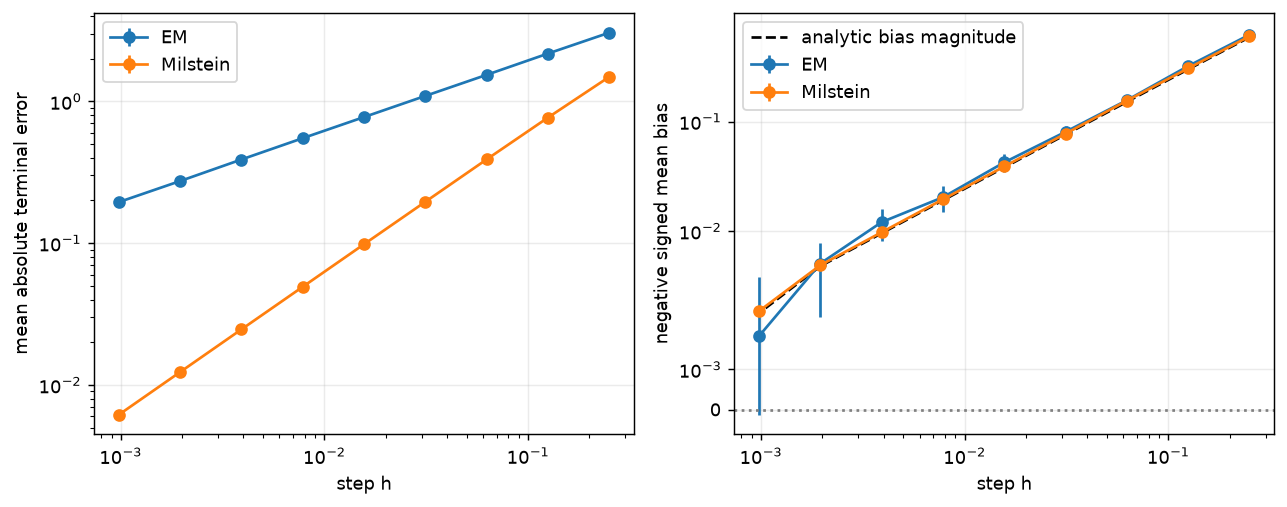
\includegraphics[width=\linewidth]{gbm_convergence.png}

\column{0.27\textwidth}
\textbf{65,536 paths}
\vspace{0.12cm}

Strong slopes:
\[
\begin{aligned}
\widehat p_{\mathrm{EM}}&=0.4975,\\
\widehat p_{\mathrm{Mil}}&=0.9972.
\end{aligned}
\]
Weak-mean slopes:
\[
\begin{aligned}
0.9610&\quad\text{EM},\\
0.9948&\quad\text{Milstein}.
\end{aligned}
\]
\end{columns}
\end{frame}
\note{
The left panel is the pathwise terminal error on log--log axes. Its slope is almost exactly one half for EM and one for Milstein. The right panel shows the signed mean bias. We used common random numbers and pointwise confidence intervals. The analytic curve confirms first-order weak bias for both methods. On the finest EM grid the confidence interval crosses zero, so we do not fit that noisy point merely to obtain a clean slope. This is the role of the uncertainty bars: they limit what we claim.
}

\begin{frame}{Histogram overlay and quantile comparison}
\footnotesize
\textbf{Benchmark:} $S_0=100$, $\mu=0.2$, $\sigma=0.3$, $T=1$;
65,536 paths, EM/Milstein with $N=32$.
\begin{center}
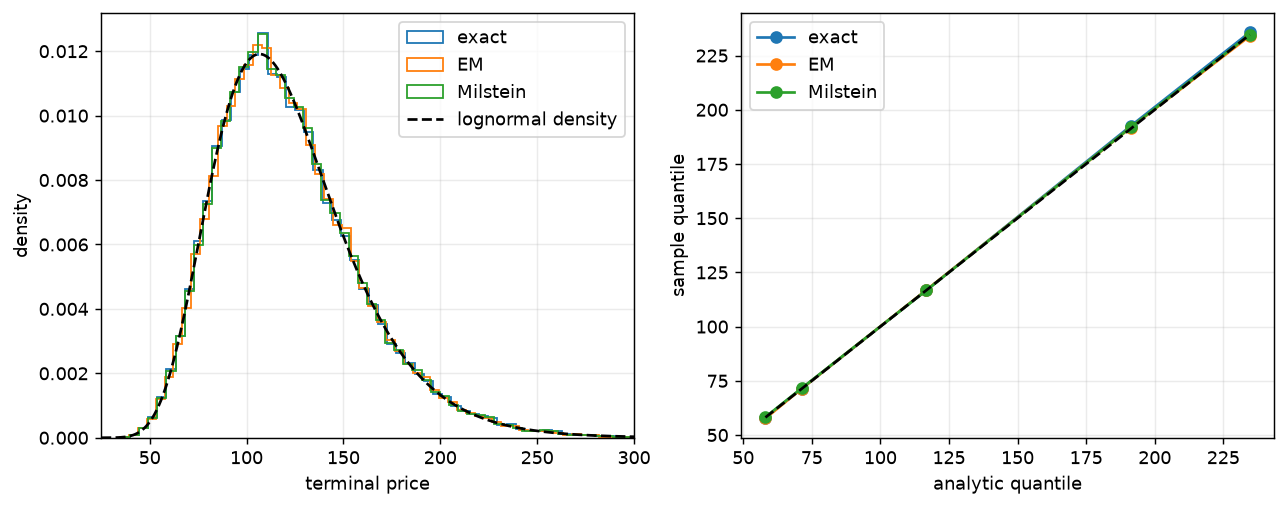
\includegraphics[width=0.92\textwidth,height=0.54\textheight,keepaspectratio]{gbm_distribution.png}
\end{center}
\begin{columns}[T,onlytextwidth]
\column{0.48\textwidth}
\textbf{Histogram:} simulated densities track the dashed exact lognormal curve,
including its right-skewed shape.
\column{0.48\textwidth}
\textbf{Quantiles:} $x=$ exact, $y=$ sampled. Points near $y=x$ show agreement;
the next table reveals small tail differences.
\end{columns}
\end{frame}
\note{
We first compare the terminal distribution visually. The left panel overlays normalised simulated histograms with the exact lognormal density. It tests the location, spread and right-skewed shape. The right panel compares sample quantiles against analytic quantiles. Agreement would put every point on the diagonal. The curves are close, but the next table makes small tail differences visible. These are distribution checks, rather than evidence that individual paths coincide.
}

\begin{frame}{Quantile comparison: centre and tails}
\small
Let $m_T=\log S_0+(\mu-\sigma^2/2)T$ and $v_T=\sigma^2T$.
Then $\log S_T\sim N(m_T,v_T)$, giving the exact density and quantile:
\[
 f(s)=\frac{\exp[-(\log s-m_T)^2/(2v_T)]}{s\sqrt{2\pi v_T}},\quad s>0,
 \qquad q_p=\exp\!\left(m_T+\sqrt{v_T}\,\Phi^{-1}(p)\right).
\]
\textbf{Simulation:} use all 65,536 terminal samples. Histogram bin height is
$count/(M\times\text{bin width})$; overlay $f(s)$ and compare sample quantiles.
\medskip

\centering
\begin{tabular}{rrrrr}
\toprule
$p$ & Exact law & Exact simulation & EM ($N=32$) & Milstein ($N=32$)\\
\midrule
0.01 & 58.106 & 58.032 & 57.644 & 58.280\\
0.05 & 71.287 & 71.348 & 71.312 & 71.565\\
0.50 & 116.766 & 116.740 & 116.877 & 116.724\\
0.95 & 191.259 & 192.508 & 191.771 & 191.907\\
0.99 & 234.645 & 235.721 & 233.999 & 234.685\\
\bottomrule
\end{tabular}
\par\medskip
\raggedright
Sample quantiles fluctuate even for exact simulation. These are descriptive
checks, not simultaneous goodness-of-fit confidence statements.
\end{frame}
\note{
This comparison combines an analytic distribution with simulation. The density and population quantiles follow from the Gaussian law of log price. The histogram comes from terminal samples, normalised by the total count and bin width. The table compares theoretical quantiles with sample quantiles for exact simulation and both numerical methods. Exact simulation also differs slightly because a finite sample has random quantiles. Agreement checks the marginal distribution but does not replace the same-path strong-error test. The preceding figure shows the histogram overlay.
}

\begin{frame}{Positivity: negative-update conditions}
\scriptsize
\setlength{\abovedisplayskip}{4pt}
\setlength{\belowdisplayskip}{4pt}
Assume $S_n>0$, $h>0$, $\sigma>0$, and $\Delta W=\sqrt h Z$, $Z\sim N(0,1)$.
\begin{columns}[T,onlytextwidth]
\column{0.48\textwidth}
\textbf{EM: a linear multiplier}
\[
 S_{n+1}=S_nF_{\mathrm{EM}},\quad
 F_{\mathrm{EM}}=1+\mu h+\sigma\sqrt h Z.
\]
\[
 S_{n+1}<0\iff
 Z<-\frac{1+\mu h}{\sigma\sqrt h}.
\]
\[
 p_{\mathrm{EM}}(h)=\Phi\!\left(-\frac{1+\mu h}{\sigma\sqrt h}\right)>0.
\]
An unbounded Gaussian lower tail means no unconditional positivity guarantee.

\column{0.48\textwidth}
\textbf{Milstein: complete the square}
\begin{align*}
 F_{\mathrm{Mil}}&=1+\mu h+\sigma\sqrt h Z
 +\tfrac12\sigma^2h(Z^2-1)\\
 &=\tfrac12\sigma^2h\left(Z+\frac1{\sigma\sqrt h}\right)^2
 +\underbrace{\tfrac12+(\mu-\tfrac12\sigma^2)h}_{c(h)}.
\end{align*}
$c(h)\ge0$: no negative multiplier.\\
$c(h)<0$: negative multipliers occur between the two roots.
\[
 z_\pm=\frac{-1\pm\sqrt{-2c(h)}}{\sigma\sqrt h},\qquad
 p_{\mathrm{Mil}}=\Phi(z_+)-\Phi(z_-).
\]
\end{columns}
\medskip
Milstein is positive almost surely for our baseline parameters, but fails for
some high-volatility, coarse-step settings. Neither scheme is unconditionally positivity-preserving.
\end{frame}
\note{
We examine one update starting from a positive price. EM becomes negative when a normal draw falls below its threshold. The normal distribution has an unbounded lower tail, so every positive step has some negative-update probability when volatility is nonzero. For Milstein, completing the square identifies the minimum multiplier c of h. If this minimum is nonnegative there are no negative updates. If it is negative, draws between the two quadratic roots cause negativity. Thus Milstein can preserve positivity for a particular parameter setting without having an unconditional guarantee across all parameters and time steps.
}

\begin{frame}{When are negative prices possible?}
\footnotesize
\setlength{\abovedisplayskip}{4pt}
\setlength{\belowdisplayskip}{4pt}
Assume $S_n>0$, $h=\Delta t>0$, $\sigma>0$, and $Z\sim N(0,1)$.
\begin{columns}[T,onlytextwidth]
\column{0.48\textwidth}
\textbf{Euler--Maruyama (EM)}
\medskip

\textbf{A negative update occurs when}
\[
 Z<-\frac{1+\mu h}{\sigma\sqrt h}.
\]
\textbf{To avoid a negative update}
\[
 Z\ge-\frac{1+\mu h}{\sigma\sqrt h}.
\]
This condition depends on the random draw. Gaussian draws have no lower bound,
so no finite $h>0$ guarantees nonnegative prices for price-space EM when $\sigma>0$.

\column{0.48\textwidth}
\textbf{Milstein}
\medskip

\textbf{Negative updates are possible when}
\[
 c(h)=\tfrac12+(\mu-\tfrac12\sigma^2)h<0.
\]
They occur for draws between the two roots shown on the preceding slide.

\textbf{To guarantee no negative updates}
\[
 \boxed{1+(2\mu-\sigma^2)h\ge0.}
\]
If $\sigma^2>2\mu$, choose
\[
 \boxed{h\le\frac1{\sigma^2-2\mu}.}
\]
If $\sigma^2\le2\mu$, every $h>0$ satisfies the condition.
\end{columns}
\medskip
\textbf{Positive-price alternative:} simulate log price and set $S_n=e^{X_n}>0$.

\end{frame}
\note{
For EM, a negative update occurs when the normal draw is below the threshold. Avoiding negativity in a particular update requires that draw to stay above the threshold. Since the Gaussian distribution has no lower bound, reducing the step cannot guarantee nonnegative EM prices when volatility is nonzero. For Milstein, the quadratic minimum gives a deterministic condition: one plus two mu minus sigma squared, multiplied by h, must be nonnegative. If sigma squared exceeds twice mu, the step must not exceed one divided by sigma squared minus twice mu. Otherwise every positive step satisfies the condition. A strict inequality makes every multiplier positive; equality permits zero only at one draw, an event of probability zero. Exponentiating a log-price simulation guarantees positive prices in exact arithmetic.
}

\begin{frame}{Non-affine stochastic volatility}
\begin{columns}[T,onlytextwidth]
\column{0.53\textwidth}
\footnotesize
\begin{align*}
\dd X_t &= \left(\mu-\frac12g(Y_t)^2\right)\dd t
          +g(Y_t)\dd W_t^{(1)},\\
\dd Y_t &= \kappa(\theta-Y_t)\dd t
          +\xi\sqrt{1+Y_t^2}\dd W_t^{(2)},\\
g(y) &= \sigma_{\min}+(\sigma_{\max}-\sigma_{\min})\ell(y),\\
\ell(y)&=\frac{1}{1+e^{-y}},\\
\dd\langle W^{(1)},W^{(2)}\rangle_t&=\rho\dd t,\\
S_t&=e^{X_t}.
\end{align*}

\column{0.38\textwidth}
\scriptsize
\renewcommand{\arraystretch}{1.18}
\begin{tabular}{@{}p{0.37\linewidth}@{\hspace{0.30em}}p{0.55\linewidth}@{}}
\toprule
$\mu=0.05$ & expected return rate\\
$\kappa=2$ & speed of reversion\\
$\theta=-0.2$ & long-run factor level\\
$\xi=0.6$ & factor noise scale\\
$\rho=-0.7$ & return-volatility relation\\
$\sigma_{\min}=0.10$ & lower volatility bound\\
$\sigma_{\max}=0.50$ & upper volatility bound\\
\bottomrule
\end{tabular}
\end{columns}
\end{frame}
\note{
The extension does not make mu random. Mu remains a constant expected return parameter. The new state Y makes volatility random. Kappa pulls Y back toward theta, while xi controls factor shocks. The logistic function g maps every real Y to a smooth positive volatility between ten and fifty percent. This prevents negative volatility and keeps the price diffusion bounded. Rho equals minus 0.7. Therefore a negative return shock tends to coincide with a positive factor shock, which raises g of Y. This reproduces the leverage-style relation often seen in equity markets. The model is non-affine because the logistic g and the square root of one plus Y squared are nonlinear state functions.
}

\begin{frame}{Why the scalar Milstein formula does not transfer}
\small
Write the correlated noises using independent Brownian motions $B_1,B_2$:
\[
W^{(1)}=B_1,
\qquad
W^{(2)}=\rho B_1+\sqrt{1-\rho^2}\,B_2.
\]
With $q(y)=\xi\sqrt{1+y^2}$, the diffusion vector fields are
\[
b_1=\begin{pmatrix}g\\ \rho q\end{pmatrix},
\qquad
b_2=\begin{pmatrix}0\\ \sqrt{1-\rho^2}\,q\end{pmatrix}.
\]
Their commutator is
\[
[b_1,b_2]
=\begin{pmatrix}-\sqrt{1-\rho^2}\,q(y)g'(y)\\0\end{pmatrix}\ne0.
\]
\end{frame}
\note{
The actual Brownian motions in the model are correlated. We construct them from two independent Brownian motions. In more than one dimension, Milstein includes cross iterated stochastic integrals. These integrals are mathematically well defined. The problem is that they cannot be reconstructed from the two endpoint increments alone when the diffusion fields do not commute. The nonzero commutator shown here proves that the simple scalar formula is incomplete. This is not because the noise becomes meaningless or uncontrollable. A full multidimensional Milstein method is possible, but it requires Lévy-area simulation and lies beyond the assigned baseline. We therefore use Euler--Maruyama for the joint system.
}

\begin{frame}{Nested Brownian grids validate the non-affine model}
\begin{columns}[c,onlytextwidth]
\column{0.65\textwidth}
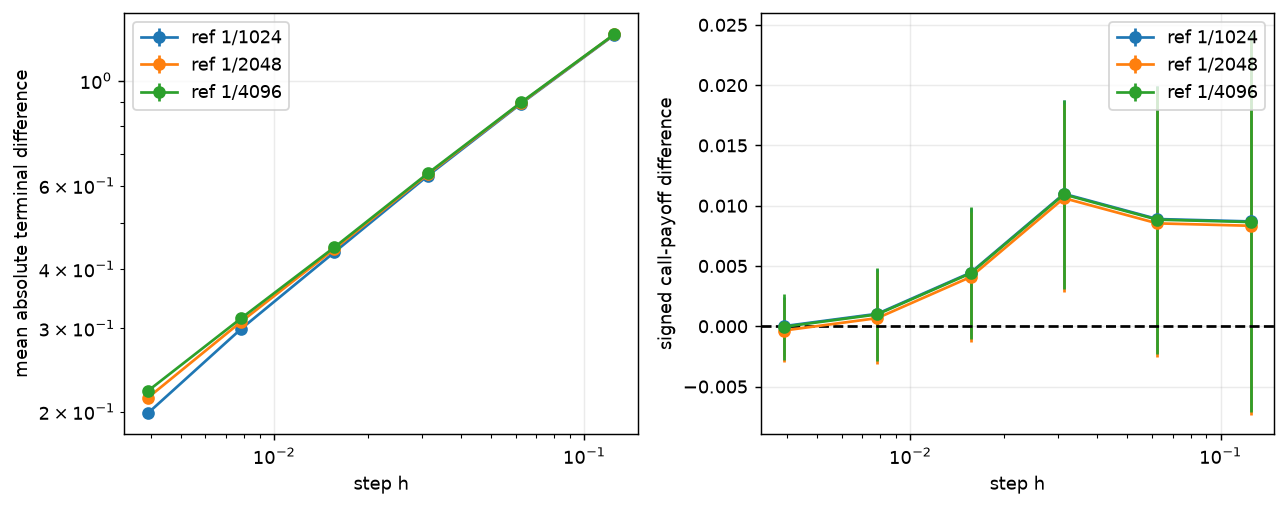
\includegraphics[width=0.84\linewidth,trim=0 0 356.40768bp 0,clip]{nonaffine_convergence.png}

\column{0.31\textwidth}
\small
Coarse increments sum fine increments:
\[
\Delta W_n^{(h)}
=\sum_{j=0}^{r-1}\Delta W_{rn+j}^{(h_f)}.
\]
\begin{itemize}
  \item 32,768 paths
  \item References: 1024, 2048, 4096 steps
  \item Finest slope: $0.5003$
\end{itemize}
\end{columns}
\end{frame}
\note{
The non-affine model has no exact transition, so we create a reference from a much finer EM grid. Coupling is essential. Each coarse Brownian increment equals the sum of the fine increments over the same interval. This means the coarse and fine solutions see the same underlying Brownian path. With independent paths, their difference would measure random path variation instead of discretisation error. We repeated the experiment with three reference grids. The strong slopes move from 0.517 to 0.506 to 0.500, which supports an empirical half-order conclusion. The call-payoff differences on the right mostly lie inside their confidence intervals, so we do not claim a weak convergence slope for this model at the current sample size.
}

\begin{frame}{Beyond the baseline: factor stability and variance reduction}
\begin{columns}[c,onlytextwidth]
\column{0.59\textwidth}
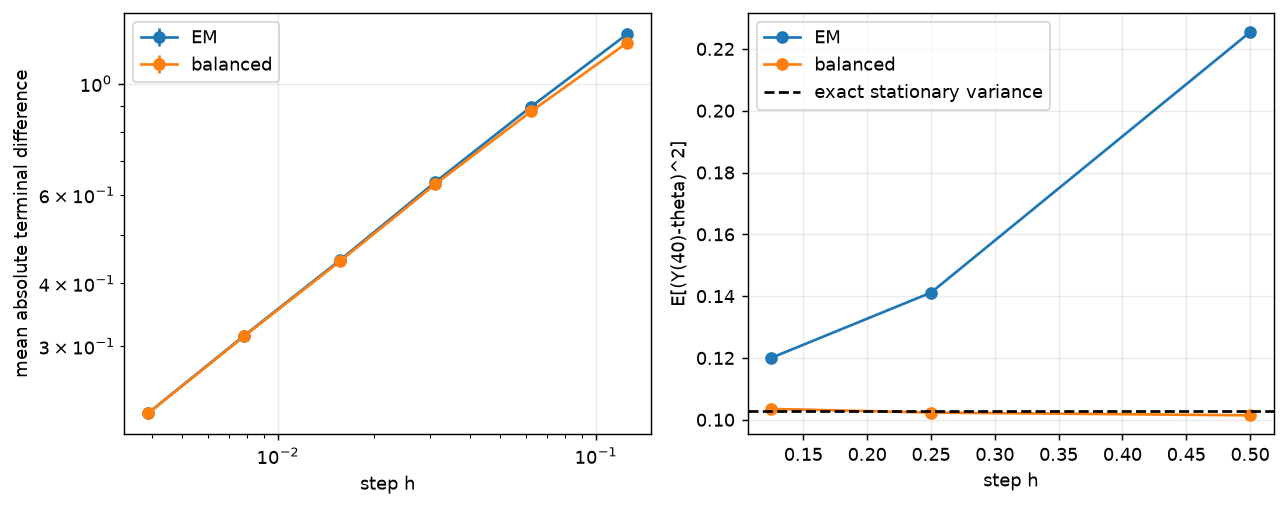
\includegraphics[width=0.95\linewidth]{extension.png}

\column{0.37\textwidth}
\small
For the call payoff $P=(S_T-K)^+$,
\[
P_{\mathrm{cv}}
=P-\widehat\beta\left(S_T-S_0e^{\mu T}\right).
\]
Independent pilot for $\widehat\beta$:
\[
\text{variance reduction}=6.23\times.
\]
At matched GBM error:
\[
N_{\mathrm{EM}}=256,
\qquad N_{\mathrm{Mil}}=16.
\]
\end{columns}
\end{frame}
\note{
We added two pieces beyond the baseline. First, the stock price has a known mean even in the non-affine model. Since the call payoff and stock price are strongly correlated, we use the centred stock price as a control variate. We estimate beta on an independent pilot sample. The variance falls by a factor of 6.23, and the standard error falls from about 0.126 to 0.051. Second, we derived a moment-balanced factor update that preserves the theoretical stationary variance and avoids the coarse-step second-moment instability of standard EM. The left panel shows this clearly. However, its one-year price error and runtime remain close to EM, so we do not claim a general speed advantage. For GBM at a common pathwise error target, Milstein needs sixteen times fewer time steps than EM, while the exact transition is still the best method.
}

\end{document}
